\section{Software Requirement Specification}

\subsection{Introduction}
	\subsubsection{Purpose}
			The purpose of this Software Requirements Specification is to describe the features, constraints and demands of a research environment for the optimal layout of graph records on disk in detail. This document is intended for both the stakeholders and the developers of the system and will be proposed to the Dr. Theodoros Chondrogiannis, the supervising postdoctoral researcher.
	\subsubsection{Scope}
			This Software system shall implement a graph record layout research environment, that consists of a graph database along with tools, that rearranges the recrods of the database based on a predefined format, measure the number of disk accesses needed to service a certain query and that provide other layouts to compare against.

    \subsubsection{Definitions, Acronyms, Abbreviations}
	\begin{longtable}{|>{\raggedright \arraybackslash}p{0.35\textwidth}||
	>{\raggedright \arraybackslash}p{0.15\textwidth}|>{\raggedright \arraybackslash}p{0.5\textwidth}|} \hline

	word & shortform & meaning \\ \hline
	database & db & a software system to store and alter data in an organized manner. \\ \hline
	Operating System & os & An operating system is system software that manages computer hardware, software resources, and provides common services for computer programs. \\ \hline
    Portable Operating System Interface & POSIX & A specification for a set of OSes that covers for example Linux, macOS and BSD-style operating systems. \\ \hline
	C Programming Language & C & a programming language. \\ \hline
	Input/Output & IO & the notion of loading and storing information to media other than RAM and CPU registers. In this document hard drive and solid state disk are meant primarily. \\ \hline
	Create, read, update, delete & CRUD & The basic database operations, that allow to create, read, update and delete a record. \\ \hline
	Databases and Information Systems & DBIS & The name of the group at the university of Konstanz, at which the software system is build. \\ \hline
	Stanford Network Analytics Project & SNAP & A porject of the university of stanford that hosts many large scale graph data sets.  \\ \hline
	Least Recently Used & LRU & A strategy when evicting pages from a pool of memory. \\ \hline
	Breadth-first Search & BFS & A graph traversal scheme, where all neighbours of the current node are visited before continuing with the next node. \\ \hline
	Depth-first Search & DFS & A graph traversal scheme, where the next node is considered before visiting all neighbours of the current node. \\ \hline
	Single Source Shortest Path & SSSP & The problem of finding the shortest path to all nodes in a graph from one source node. \\ \hline
	\dots & \dots & \dots \\ \hline
	\hline
	\end{longtable}

	\subsubsection{Overview}
		In the second chapter several conditions, assumptions and circumstances will be mentioned, that help charachterizing the software's special use case. In the thrid chapter the concrete requirements are listed.

		
\subsection{Overall description}
	\subsubsection{Product Perspective}
		The product shall rely on functions of unixoid OSes. 
		That is it uses the interfaces specified by the OpenGroup in the POSIX.1-2017 specification (also called IEEE Std 1003.1-2017)~\autocite{posix}.
		There are no relations to other software systems than the operating system during the runtime of the environment.

	\subsubsection{Product Functions}
	The product shall support different tasks in graph record layout research: 
		\begin{enumerate}
		 \item Import data into a graph database.
		 \item Query the database with a certain fixed function.
		 \item Rearange the record layout on disk with a layout given in a specific format.
		 \item Monitor the number of disk IOs.
		 \item Monitor the caching behaviour.
		 \item Provide interfaces for the implementation of new layout methods.
		 \item Provide a interfaces to ease the implementation of new queries.
		\end{enumerate}
		
        This shall be done using a graph database, that shall save related information to disk and load them into a cache on access, as well as support the common CRUD functionality. \\
        

	\subsubsection{User Characteristics}
		The potential users are the staff and student assistants of the DBIS group. Therefore standard user will have technical knowldege, and have visited at least a basic course on databases. Futher the users are able to program in C.
		There are three different types of users of this research environment: \\
		\begin{itemize}
			\item Researchers: Implements new layout method, benchmarks the result of the method against other layouts, visualizes the result of the benchmark. Should at least know the theory of how records are stored.
			
		 	\item Supervisors: Works on the administration and coordination of the project. Eventually hires other researchers and developers. Also a researcher.
		 	\item (Future) Developers: Uses the existing framework to extend the functionality, for example to implement additional queries of a different type, add new features like storing properties and similar things. Needs to know details of database architecture and implementation, more advanced C programming and some software engineering.
		\end{itemize}
		\begin{center}
		 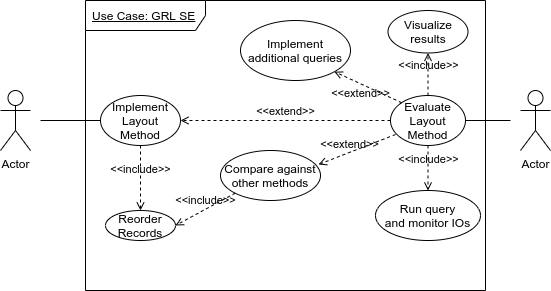
\includegraphics[keepaspectratio,width=\textwidth]{img/use_case.png}
		\end{center}

	\subsubsection{Constraints}
		\begin{itemize}
			\item The database is expected to be run on a standard notebook and desktop machine, that is it needs to run without momory-related errors on a machine with 8 GiB RAM, no matter the data set size.
		\end{itemize}

	\subsubsection{Assumptions and Dependencies}
		The environment supports only POSIX-compliant OSes.


\subsection{Specific Requirements}

	\subsubsection{External interfaces}
	The POSIX interfaces. \\
	The data format of some of the SNAP data sets. \\

	\subsection{Functional requirements}
\begin{enumerate}[label*=\arabic*]
\item Data Storage and IO \\
    The system shall
	\begin{enumerate}[label*=\arabic*]
	\item store a graph $G$ consisting of nodes and edges $(V, E)$.
	\item store the records in a file on disk.
    \item be able to grow and shrink the size of the file that is used.
    \item be able to read from disk.
    \item be able to write information to disk.
	\end{enumerate}
	
\item Data Caching and Memory  \\
    The system shall
	\begin{enumerate}[label*=\arabic*]
	\item not exceed a certain memory limit for both pages from disk and memory requirements from queries.
	\item split an amount of memory into frames.
	\item load data from disk into a frame on request.
	\item maintain information on unused frames.
	\item maintain a mapping from loaded data to frames.
	\item evict data from memory when the memory limit is hit
	\item be able to prefetch by reading more data than required in a neighbourhood
    \item be able to monitor the numer of overall disk accesses.
	\item be able to monitor the number of disk accesses that are necessary, if only a certain limited amount of memory is available.
	\item be able to monitor the cache hit rate.
	\item be able to monitor the prefetch hit rate.
	\end{enumerate}

\item Data Access \\
    The system shall
	\begin{enumerate}[label*=\arabic*]
    \item be able to calculate the location in the file of nodes and relationships efficiently
    \item keep track of free record slots on disk.
	\item be able to create, read, update and write nodes.
	\item be able to create, read, update and write relationships.
	\item provide an interface to easily retrieve and traverse data.
    \item provide functions to retrieve common informations about nodes and relationships, like the node degree.
	\end{enumerate}

\item Queries \\
    The system shall
	\begin{enumerate}[label*=\arabic*]
	\item implement the most basic traversal schemes --- BFS and DFS.
	\item implement Dijksta's algorithm for finding all shortest paths from a single source (SSSP).
	\item implement the A$^*$ algorithm for the shortest path problem.
	\item implement the ALT algorithm for the shortest path problem.
	\item provide data structures for the results of the above algorithms.
	\item implement the Louvain method for community detection.
	\item implement a random walk.
	\item be able to import a set of standard data sets from the SNAP data set collection.
	\end{enumerate}

\item Layout Tools \\
    The system shall
\begin{enumerate}[label*=\arabic*]
	\item provide a function to generate a randomized record layout.
	\item provide functions to reorganize the record layout on disk, given updated record IDs.
	\item provide a function to reorganize the relationships given a layout of the vertices.
	\item provide a function to sort the incidence list structure after reorganizing the record structure.
\end{enumerate}

\item Layout Methods \\
    The system shall
\begin{enumerate}[label*=\arabic*]
	\item implement one static and one dynamic history-based layout method for a static database.
	\item provide an interface for implementing new layout methods.
\end{enumerate}

\item Visualization Tools \\
    The system shall
\begin{enumerate}[label*=\arabic*]
    \item provide functions to visualize and visually compare the data that was monitored by the caching functionality.
\end{enumerate}
\end{enumerate}
\begin{center}
 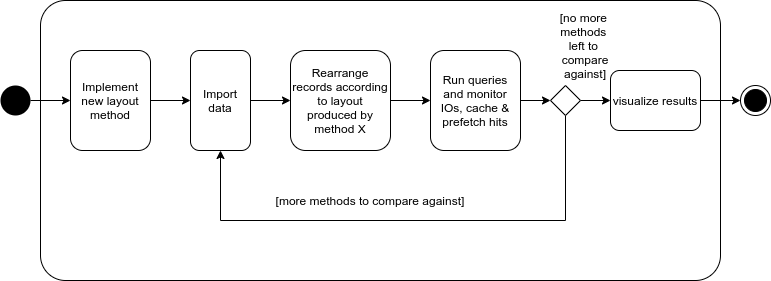
\includegraphics[keepaspectratio, width=\textwidth]{img/activity.png}
\end{center}


\subsection{Performance Requirements}
\begin{enumerate}[label*=\arabic*]
		\item The system shall work with limited RAM resources even for very large datasets.
\end{enumerate}

\subsection{Software System Attributes}
\begin{enumerate}[label*=\arabic*]
		\item Maintainability
		\item Extensibility
		\item Correctness
\end{enumerate}





      

      
